% !TeX spellcheck = cs_CZ
%{\tikzset{external/prefix={tikz/FYZII/}}
% \tikzset{external/figure name/.add={ch41_}{}}
%---------------------------------------------------------------------------------------------------
% file fey2ch41.tex
%---------------------------------------------------------------------------------------------------
%=========================== Kapitola Proudění "mokré vody" ========================================
\setchaptertoc
\chapter{Proudění \uv{mokré vody}}\label{fyz:IIchapXLI}

  \section{Viskozita}\label{fyz:IIchapXLIsecI}
    V předcházející kapitole jsme probrali chování vody, přičemž jsme zanedbali jev viskozity. Nyní 
    bychom se chtěli podívat na skutečné chování tekutin. Kvalitativně popíšeme, jak se tekutiny 
    chovají za nejrůznějších okolností, abychom získali o tématu jistou představu. Ačkoliv si 
    ukážeme několik složitých rovnic a řekněme o některých složitých jevech, není naším cílem, 
    abychom se naučili všechno. V jistém smyslu je tato kapitole „kulturní vsuvkou“, která nám má 
    poskytnout představu o tom, jak vypadá svět. Pouze jedna věc by se vyplatila naučit, a to 
    jednoduchá definici viskozity, k níž se dostaneme za chvíli. Vše ostatní je tu pro naše 
    pobavení.
    
    V předcházející kapitole jsme zjistili, že zákony pohybu tekutiny jsou obsaženy v této rovnici:
    \begin{equation}\label{fyz:eq569}
      \pder{\bm{v}}{t} + (\bm{v}\cdot\symbf{\nabla})\times\bm{v} 
          = -\dfrac{\symbf{\nabla}p}{\varrho} -\symbf{\nabla}\varphi + 
             \dfrac{\bm{f_{visk}}}{\varrho}.
    \end{equation}
    
    V našem přiblížení „suché“ vody jsme vynechali poslední člen a zanedbali tak všechny viskózní 
    efekty. Kromě toho jsme občas přidali další přiblížení tím, že jsme tekutinu považovali za 
    nestlačitelnou; tehdy jsme měli dodatečnou rovnici
    \begin{equation*}
      \symbf{\nabla}\cdot\bm{v} = 0.
    \end{equation*}
    Poslední přiblížení je často velmi dobré, zvláště když jsou rychlosti proudění mnohem menší než 
    rychlost zvuku. Ale ve skutečných tekutinách nemůžeme téměř nikdy zanedbat vnitřní tření, které 
    nazýváme viskozitou; většina zajímavých jevů, k nimž dochází, s ní tak nebo onak souvisí. 
    Například jsme viděli, že v „suché“ vodě se cirkulace nikdy nemění: byla-li nulová na počátku, 
    nikdy nebude jiná. Naproti tomu cirkulace v tekutinách se objevuje každou chvíli. Musíme proto 
    naši teorii poopravit.
    
    Začneme důležitým experimentálním faktem. Když jsme se zabývali prouděním „suché“ vody kolem 
    válce, tzv. „potenciálním prouděním“, nebyl důvod nedovolit vodě, aby měla tangenciální 
    rychlost vzhledem k povrchu válce; pouze normálová složka musela být nulová. Nezvážili jsme 
    možnost, že může existovat smyková síla mezi tekutinou a pevnou látkou. Ukazuje se (ačkoliv to 
    není vůbec samozřejmé), že ve všech případech, které byly experimentálně prověřeny, \emph{je 
    rychlost tekutiny u povrchu pevné látky přesně nulová}. Už jsme si bezpochyby všimli, že na 
    lopatce ventilátoru se nasbírá tenká vrstva prachu a že na ní zůstane i po té, co provětrávala. 
    Stejný jev uvidíme dokonce i na velkém ventilátoru v aerodynamickém tunelu. Proč vzduch 
    neodvěje prach? Přesto, že lopatka ventilátoru se vzduchem pohybuje velkou rychlostí, rychlost 
    vzduchu vzhledem k lopatce klesá u jejího povrchu k nule. Nejmenší částečky prachu proto 
    zůstávají na místě.\footnote{Z desky stolu můžeme sfouknout velké prachové částečky, ale ne ty 
    nejmenší. Větší částečky totiž vyčnívají do proudu vzduchu} Musíme naši teorii pozměnit tak, 
    aby byla ve shodě s experimentální skutečností, že ve všech normálních tekutinách mají molekuly 
    blízko pevného povrchu (vzhledem k povrchu) nulovou rychlost.\footnote{Lze si představit 
    podmínky, za nichž toto tvrzení neplatí: sklo je teoreticky „tekutina“, ale zaručeně lze 
    dosáhnout toho, aby klouzalo po povrchu oceli. I toto naše tvrzení tedy má své hranice, za 
    nimiž přestává platit.}
    
    \begin{figure}[ht!] %\ref{fyz:fig535}
      \centering
      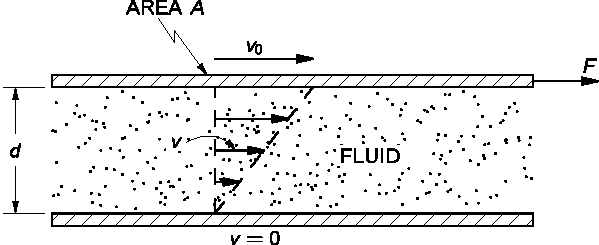
\includegraphics[width=0.7\linewidth]{fyz_fig535.pdf}
      \caption{Unášení viskózní tekutiny mezi dvěma rovnoběžnými deskami
               (\cite[s.~760]{Feynman02})}
      \label{fyz:fig535}
    \end{figure}
    
    Původně jsme charakterizovali tekutinu tím, že přiložíme-li k ní (libovolně malé) smykové 
    napětí, tekutina se mu poddá. Teče. Ve statických situacích neexistují smyková napětí. 
    Ale dříve než je dosaženo rovnováhy, pokud ještě na tekutinu působíme, mohou smykové síly 
    existovat. Viskozita právě popisuje smykové síly, které existují v pohybující se tekutině. 
    Abychom našli míru smykových sil po dobu pohybu tekutiny, přestavíme si pokus následujícího 
    typu. Představme si, že máme dvě pevné rovinné desky, mezi nimiž je voda (obr. 
    \ref{fyz:fig535}), přičemž jednu z nich udržujeme v klidu a druhou pohybujeme rovnoběžně malou 
    rychlostí \(v_0\). Změříme-li sílu, která je potřebná k tomu, abychom horní desku udrželi v 
    pohybu, zjistíme, že je úměrná ploše desek a \(v_0/d\), přičemž \(d\) je vzdálenost mezi 
    deskami. Smykové napětí \(F/S\) je tedy úměrné \(v_0/d\):
    \begin{equation*}
      \dfrac{F}{S} = \eta\dfrac{v_0}{d}.
    \end{equation*}
    Konstanta úměrnosti \(\eta\) se nazývá \textbf{dynamická viskozita}. 
    
    Ve složité situaci si vždy můžeme vybrat malý tenký hranol vody, jehož stěny jsou rovnoběžné s 
    prouděním (obr. \ref{fyz:fig536}). Smyková síla, která působí na tento hranolek, je
    \begin{equation}\label{fyz:eq570}
      \dfrac{\Delta F}{\Delta S} = \eta\dfrac{\Delta v_x}{\Delta y} = \eta\pder{v_x}{y}.
    \end{equation}
    \begin{figure}[ht!] %\ref{fyz:fig536}
      \centering
      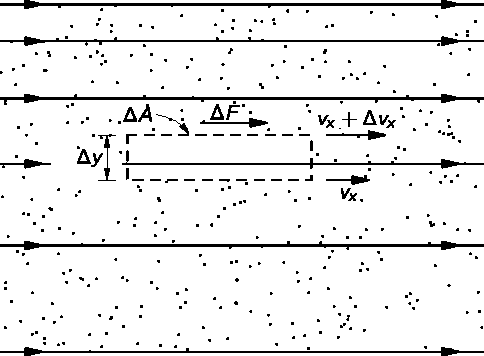
\includegraphics[width=0.7\linewidth]{fyz_fig536.pdf}
      \caption{Smykové napětí ve viskózní tekutině
               (\cite[s.~760]{Feynman02})}
      \label{fyz:fig536}
    \end{figure}
    Zde je \(\pder{v_x}{y}\) rychlost změny deformace ve smyku, kterou jsme definovali v kapitole 
    \ref{fyz:IIchapIIXL}, takže v tekutině je smykové napětí úměrné \emph{rychlostí změny} smykové 
    deformace.

    V obecném případě píšeme
    \begin{equation}\label{fyz:eq571}
      S_{xy} = \eta\left(\dfrac{\Delta v_y}{\Delta x} + \dfrac{\Delta v_x}{\Delta y}\right)
    \end{equation}
    
    Rotuje-li tekutina rovnoměrně, je \(\dfrac{\Delta v_x}{\Delta y}\) opačné k \(\dfrac{\Delta 
    v_y}{\Delta x}\) a \(S_{xy}\). je nulové. Musí to tak být, neboť v rovnoměrně rotující tekutině 
    nejsou smyková napětí. (Něco podobného jsme požadovali i při definici \(e_{xy}\), v kapitole 
    \ref{fyz:IIchapIXL}.) Samozřejmě, i pro \(S_{yz}\) a \(S_{zx}\) platí odpovídající výrazy.
    
    \begin{figure}[ht!] %\ref{fyz:fig537}
      \centering
      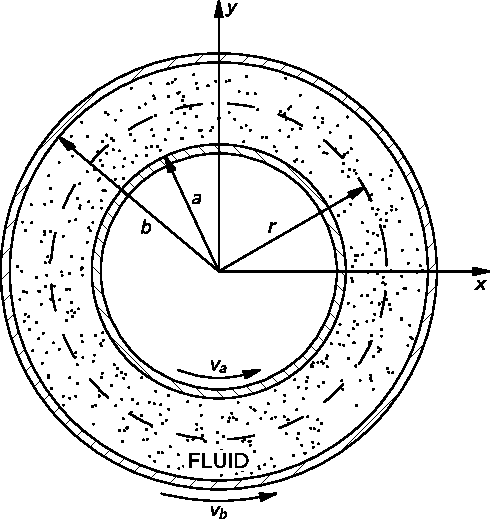
\includegraphics[width=0.7\linewidth]{fyz_fig537.pdf}
      \caption{Proudění tekutiny mezi dvěma souosými válci, které se otáčejí různými úhlovými 
               rychlostmi.
               (\cite[s.~760]{Feynman02})}
      \label{fyz:fig537}
    \end{figure}
    
  \section{viskózní proudění}\label{fyz:IIchapXLIsecII}
    
  \section{Reynoldsovo číslo}\label{fyz:IIchapXLIsecIII}
  
  \section{Obtékání kruhového válce}\label{fyz:IIchapXLIsecIV}
  
    \begin{figure}[ht!] %\ref{fyz:fig538}
      \centering
      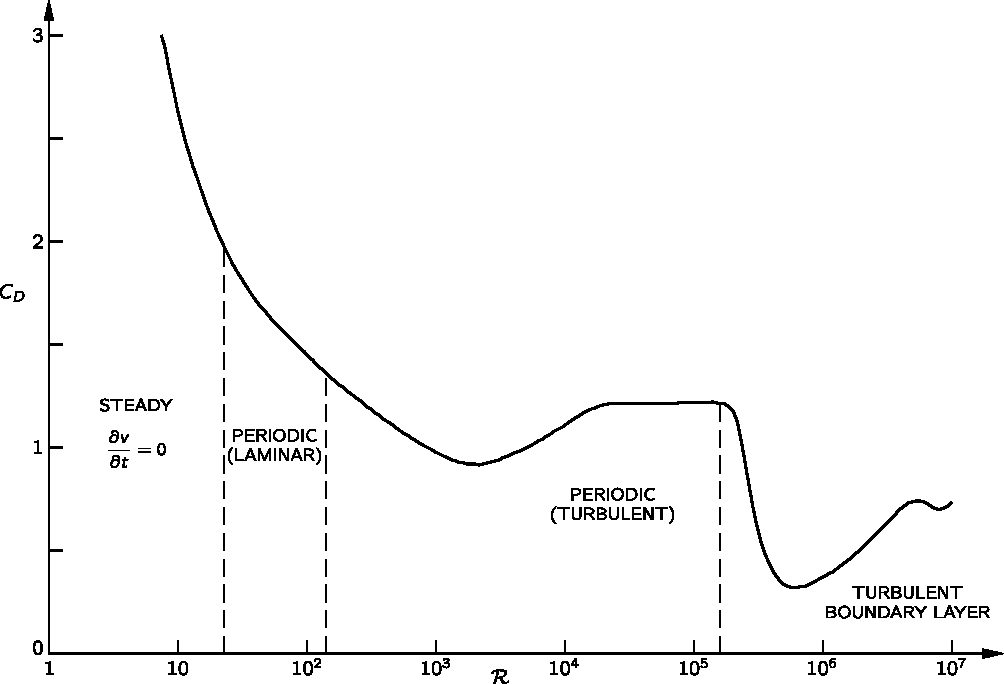
\includegraphics[width=1\linewidth]{fyz_fig538.pdf}
      \caption{Součinitel odporu \(C_D\) kruhového válce jako funkce Reynoldsova čísla.
               (\cite[s.~766]{Feynman02})}
      \label{fyz:fig538}
    \end{figure}
     
    \begin{figure}[ht!] %\ref{fyz:fig539}
      \centering
      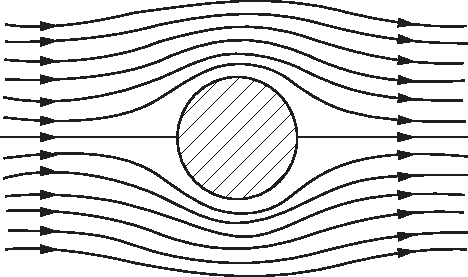
\includegraphics[width=0.7\linewidth]{fyz_fig539.pdf}
      \caption{Viskózní proudění kolem kruhového válce při malých rychlostech
              (\cite[s.~707]{Feynman02})}
      \label{fyz:fig539}
    \end{figure}   

    \begin{figure}[hb!] %\ref{fyz:fig540}
      \centering
      \subcaptionbox{\label{fyz:fig540a}}{\luafigure[0.9]{fyz_fig540a.pdf}}  \newline
      \subcaptionbox{\label{fyz:fig540b}}{\luafigure[0.9]{fyz_fig540b.pdf}}  \newline
      \subcaptionbox{\label{fyz:fig540c}}{\luafigure[0.9]{fyz_fig540c.pdf}}  \newline
      \subcaptionbox{\label{fyz:fig540d}}{\luafigure[0.9]{fyz_fig540d.pdf}}  \newline
      \subcaptionbox{\label{fyz:fig540e}}{\luafigure[0.9]{fyz_fig540e.pdf}}  
      \caption{Obtékání válce při různých Reynoldsových číslech
               (\cite[s.~768]{Feynman02}).}
      \label{fyz:fig540}
    \end{figure}

    \begin{figure}[ht!] %\ref{fyz:fig541}
      \centering
      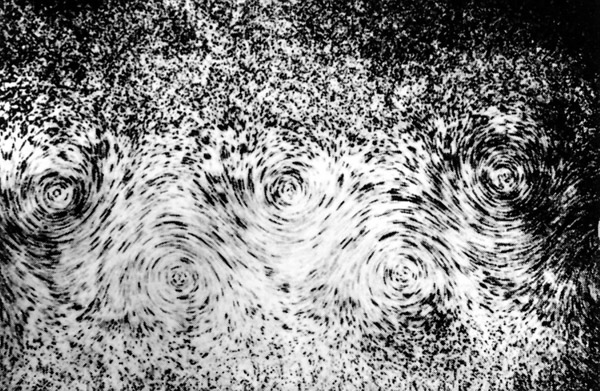
\includegraphics[width=0.7\linewidth]{fyz_fig541.jpg}
      \caption{Fotografie Ludwiga Prandlta zachycuje \uv{vírovou cestu} v proudu za válcem
               (\cite[s.~707]{Feynman02})}
      \label{fyz:fig541}
    \end{figure}
    
  \section{Limita nulové viskozity}\label{fyz:IIchapXLIsecV}
  \section{Couettovo proudění}\label{fyz:IIchapXLIsecVI}

    \begin{figure}[hb!] %\ref{fyz:fig542}
      \centering
      \subcaptionbox{\label{fyz:fig542a}}{\luafigure[0.45]{fyz_fig542a.pdf}}
      \subcaptionbox{\label{fyz:fig542b}}{\luafigure[0.45]{fyz_fig542b.pdf}}
      \caption{Různé druhy proudění kapaliny mezi dvěma průhlednými rotujícími válci
               (\cite[s.~770]{Feynman02}).}
      \label{fyz:fig542}
    \end{figure}
  
    \begin{figure}[hb!] %\ref{fyz:fig543}
      \centering
      \subcaptionbox{\label{fyz:fig543a}}{\luafigure[0.45]{fyz_fig543a.pdf}}
      \subcaptionbox{\label{fyz:fig543b}}{\luafigure[0.45]{fyz_fig543b.pdf}}  \newline
      \subcaptionbox{\label{fyz:fig543c}}{\luafigure[0.45]{fyz_fig543c.pdf}}  
      \caption{Proč se proudění rozloží na pásy
               (\cite[s.~770]{Feynman02}).}
      \label{fyz:fig543}
    \end{figure}

  \section{Příklady a cvičení}\label{fyz:IIchapXLIsecVII}


  \todo[inline]{Kapitola fey2ch41 je nedodělaná, obsahuje pouze obrázky}
%} %tikzset
%---------------------------------------------------------------------------------------------------